
\documentclass[11pt,letterpaper]{article}
\usepackage{amssymb,amsmath}
\usepackage{mathrsfs}
\usepackage{epsfig}
\usepackage{anysize}
\usepackage{verbatim}
\usepackage[latin1]{inputenc}
\usepackage[spanish]{babel}
%\input{macrosal}
\title{Resolviendo el problema del TSP con Recocido Simulado}
\author{V�ctor Zamora Guti�rrez}
\date{}
\begin{document}
\maketitle
\thispagestyle{empty}
El recocido simulado es una heur�stica de optimizaci�n combinatoria que sirve para resolver problemas NP duros. En esta ocasi�n, utilizamos dicha heur�stica para resolver un caso modificado del Traveling Salesman Problem (TSP): dado un conjunto de ciudades, encontrar el camino de menor peso que pase por todas las ciudades exactamente una vez.
\section{Para correr el programa}
Para correr el programa, se necesita una distribuci�n de Linux con java 8, ant y sqlite3.
Para instalar dichos programas desde ArchLinux, ejecutar:
\begin{verbatim}
$sudo pacman -S jre8-openjdk
$sudo pacman -S jdk8-openjdk
$sudo pacman -S apache-ant
$sudo pacman -S sqlite
\end{verbatim}
Teniendo esto, desde la carpeta ra�z del proyecto (la que tiene el build.xml) ejecutar:
\begin{verbatim}
$ant tsp.jar
$java -jar tsp.jar <semilla> <ciudades>
\end{verbatim}
Donde semilla es la semilla con la que se quiere correr el recocido y ciudades es un archivo que contiene una lista de ids de ciudades, separadas por una coma y un espacio.
Por ejemplo, ciudades puede tener la siguiente l�nea:
\begin{center}
1, 5, 9, 12, 16, 22, 23, 29, 30, 31, 39, 48, 52, 56, 58, 62, 65, 66, 70, 75, 80, 84, 86, 90, 92, 94, 95, 101, 107, 117, 119, 122, 133, 135, 143, 144, 146, 147, 150, 158, 159, 160, 166, 167, 176, 178, 179, 185, 186, 188, 190, 191, 194, 198, 200, 203, 207, 209, 213, 215, 216, 220, 221, 224, 227, 232, 233, 235, 238, 241, 244, 248, 250, 254, 264, 266, 274, 276
\end{center}

\section{Ejecuci�n en una gr�fica}
Mostraremos la ejecuci�n del algoritmo de Warshall en la siguiente gr�fica:\\
\begin{center}
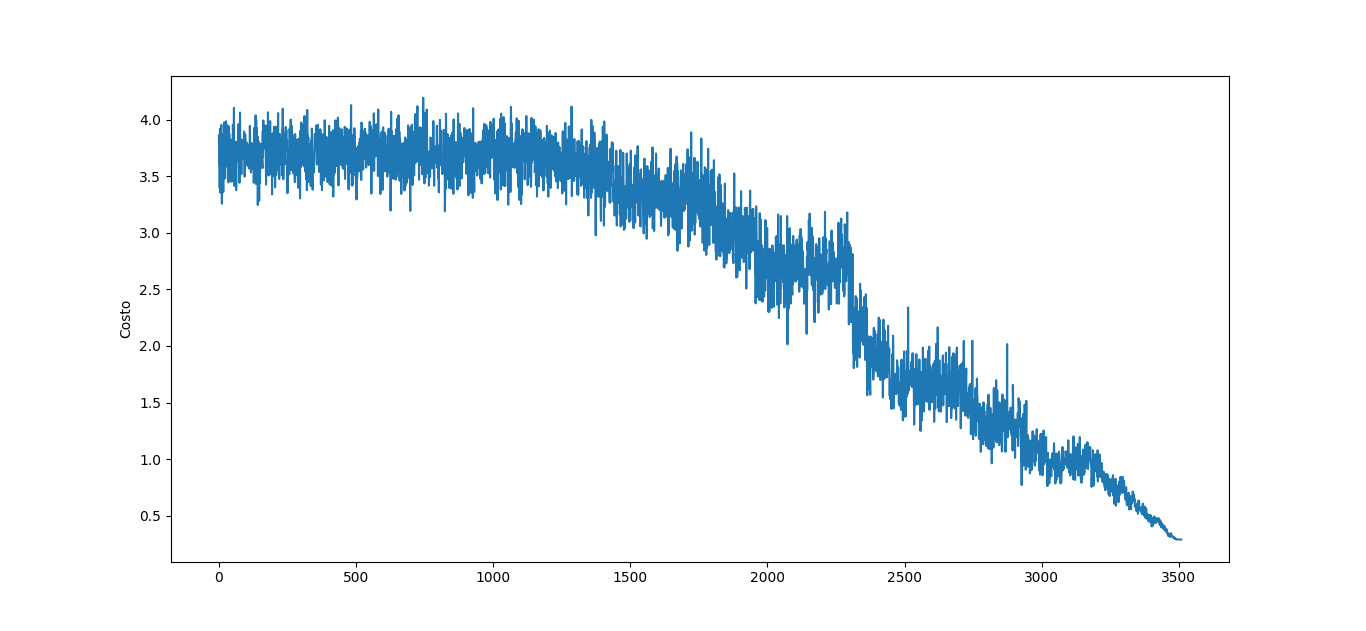
\includegraphics[width=5cm, height=4cm]{grafica}
\end{center}
\paragraph{Paso 1}
Primero tomamos a 1 como pivote. Recordemos que lo que queremos es relacionar dos elementos que est�n indirectamente relacionados por medio del 1. En este caso, los �nicos nodos que cumplen esto son 2 y 4, como se muestra a continuaci�n:\\
Sin embargo, 2 y 4 ya est�n relacionado por lo que no hacemos nada.
\paragraph{Paso 2}
Tomamos a 2 como pivote. En este caso tenemos que 3 est� relacionado con 2, por lo que debemos relacionar a 3 con todos los elementos con los que 2 est� relacionado (en este caso son 1 y 4):
\paragraph{Paso 3}
Tomamos a 3 como pivote. Como 4 se relaciona con 3, debemos relacionar a 4 con todos los vecinos de 3 (en este caso, con todos los nodos excepto 3).
\paragraph{Paso 4}
Por �ltimo, tomamos a 4 como pivote. Como 1, 2 y 3 se relacionan con 4, los tenemos que relacionar con los vecinos de 4 (en este caso, todos los nodos).
Y tenemos la gr�fica de la cerradura transitiva.
\section{Ejecici�n en una matriz}
Las relaciones tambi�n pueden representarse como matrices (y de hecho, el algoritmo originalmente se hace sobre una matriz). A continuaci�n, veremos la ejecuci�n del algoritmo en la siguiente matriz de relaci�n.
\paragraph{Paso 1}
Tomamos al primer elemento como pivote. Primero nos fijamos en la fila 1. Esta s�lo tiene 1 en la columna 4 y 0 en las dem�s. Luego nos fijamos en las dem�s filas. A las que tengan un 1 en la columna 1, les agregamos todos los 1's de la fila 1(en este caso, s�lo agregamos el 1 de la columna 4). Despu�s de la primera iteraci�n, la matriz queda as�:
N�tese que aunque la fila 3 tiene un 1 en la columna 1, no se le agregan 1's porque ya tiene el 1 de la columna 4.
\paragraph{Paso 2}
Ahora tomamos al segundo elemento como pivote. La segunda fila tiene 1's en las columnas 1, 3 y 4. Nos fijamos en las dem�s filas y de nuevo, a las que tengan un 1 en la columna 2, les agregamos 1's en las columnas 1, 3 y 4. La matriz queda as�:
Como ninguna fila tiene un 1 en la columna 2, no hubo cambios.
\paragraph{Paso 3}
Tomamos al tercer elemento como pivote. La fila 3 tiene 1's en las columnas 1 y 4. Ahora nos fijamos en las filas que tengan 1 en la columna 3 y les agregamos los 1's de las columnas 1 y 4.
\paragraph{Paso 4}
Por �ltimo, tomamos al cuarto elemento como pivote. La cuarta fila tiene 1's en las columnas 1, 3 y 4. Nos fijamos en todas las filas que tengan un 1 en la columna 4 y les agregamos estos elementos:
Como ya no quedan elementos para usar como pivotes, ya tenemos la cerradura transitiva:
\end{document}
 
 
